\documentclass[../DefinizioneDiProdotto_v2.0.0.tex]{subfiles}

\begin{document}

\section{Diagrammi di attività}
In questa sezione viene descritta e rappresentata tramite un diagramma di attività UML la sequenza di azioni del FlowModule.

\subsection{FlowModule}
Nel seguente diagramma viene riportato il flusso di azioni che l'AV esegue ogni volta che riceve una risposta ad una domanda.

\begin{figure}[!h]
	\centering
	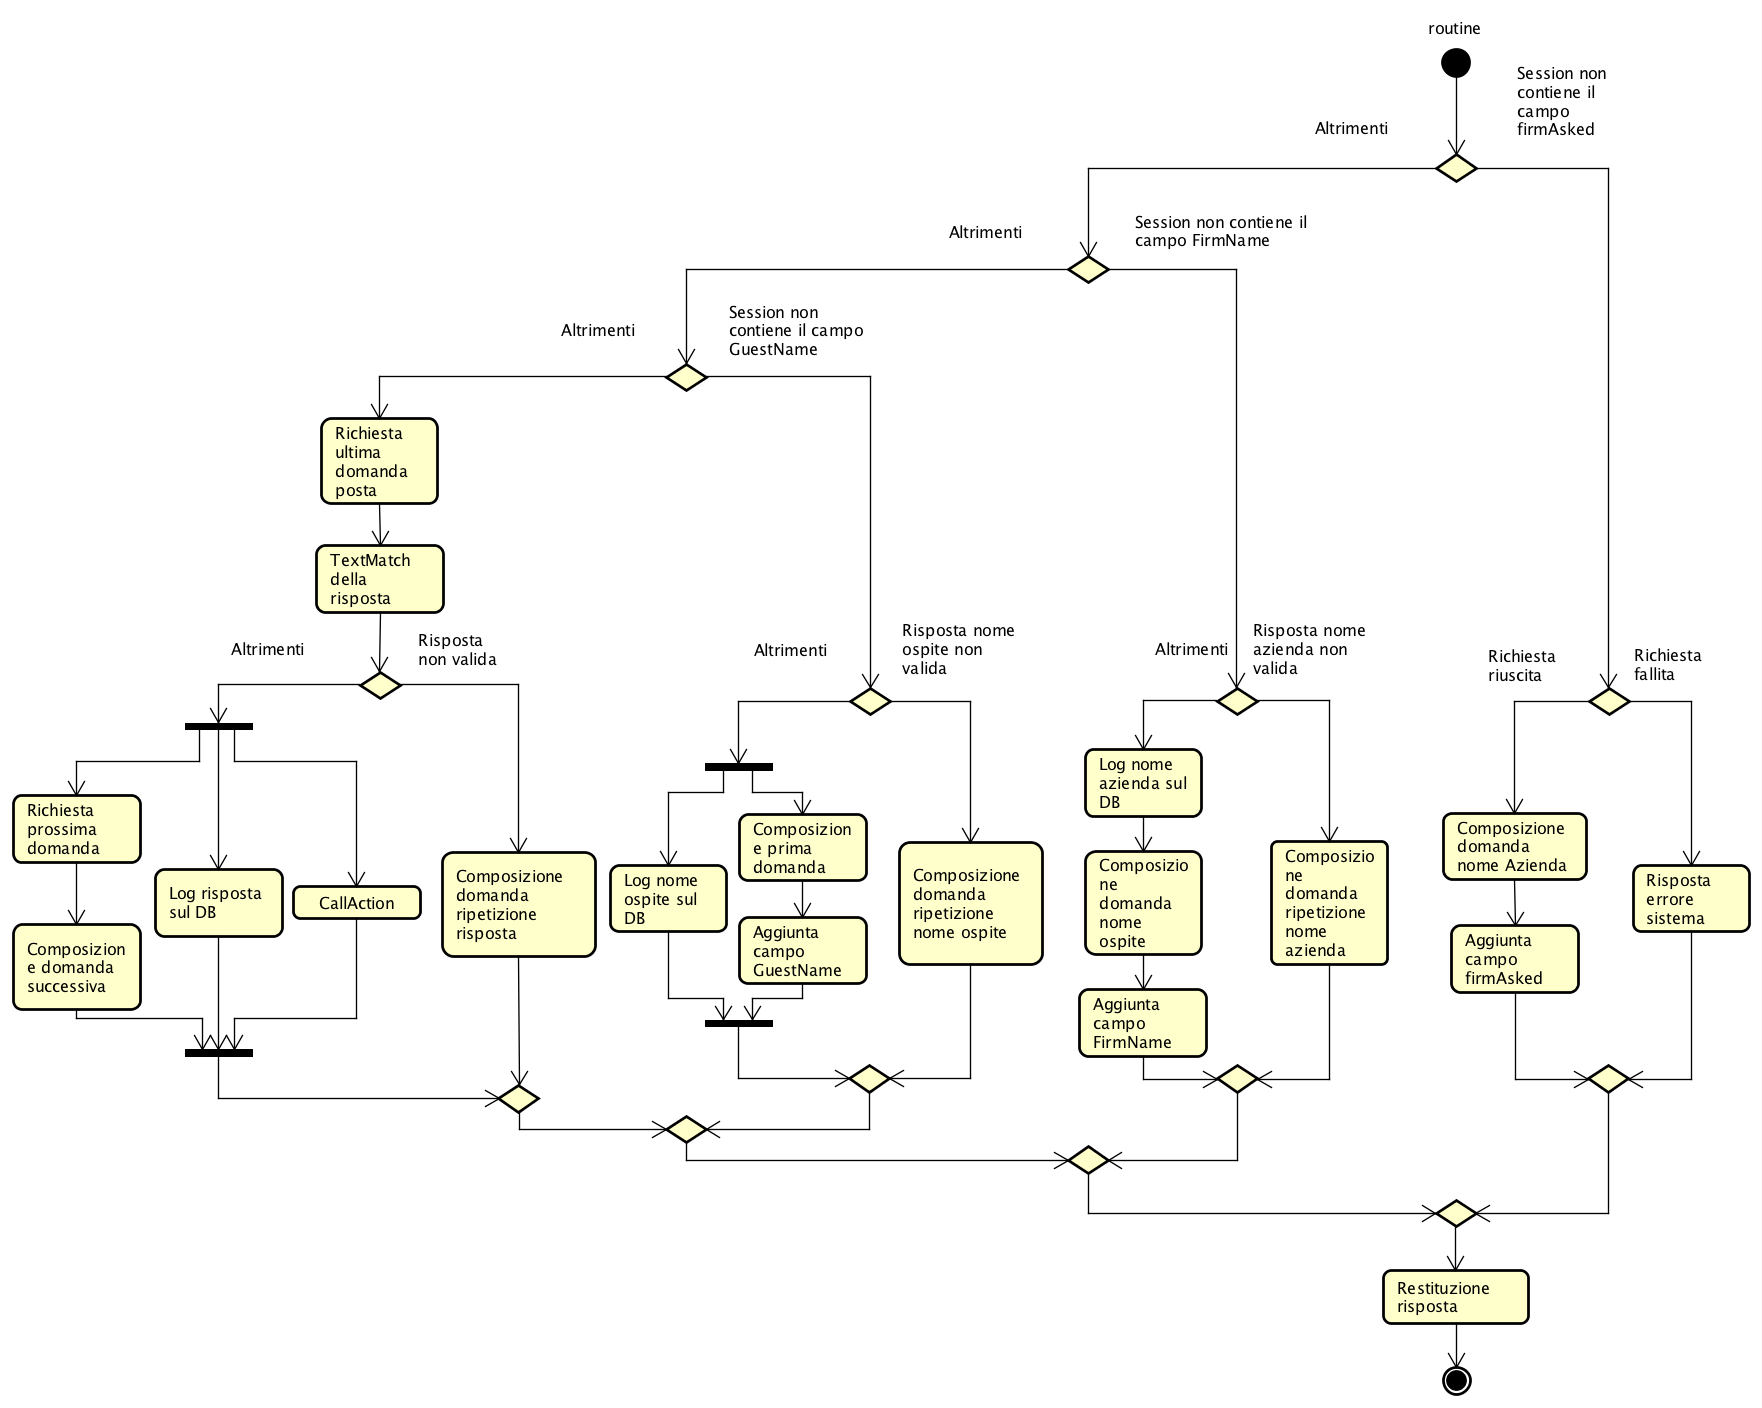
\includegraphics[scale=0.3]{DiagrammiFlusso/FlussoFlowModule.png}
	\caption{Diagramma di attività - \texttt{FlowModule}}
\end{figure}
\begin{description}
	\item [Descrizione] Il diagramma di attività inizia con la verifica, da parte dell'AV, se è già stato chiesto il nome dell'azienda all'ospite. Nel caso in cui non sia già stato fatto si procederà con la somministrazione della domanda e con l'attesa di una riposta, se la formulazione della domanda non va a buon fine verrà inviato un errore. Se, invece,  l'azienda di appartenenza è già stata chiesta si procederà con la verifica del nome di quest'ultima e se è già compreso o meno dall'AV. In quest'ultimo caso esso verrà chiesto e se a sua volta sarà compreso si passerà alla richiesta del nome dell'ospite e alla sua registrazione, in negativo la domanda verrà ripetuta. Nel caso in cui sia già stato compreso il nome dell'azienda, ma non il nome dell'ospite allora quest'ultimo verrà richiesto e contemporaneamente salvato nel database. Se invece il nome dell'ospite era già stato compreso allora si richiederà l'ultima domanda posta, verrà verificato che la risposta corrisponda ad una di quelle accettate dal sistema, se ciò avviene verrà salvata la risposta data, eseguita la rispettiva azione e somministrata la successiva domanda. Invece, se la risposta non corrisponde ad una di quelle accettate, si procederà alla ripetizione della domanda posta e si attenderà una risposta.
\end{description}

\end{document}
